\section{Probing and Causal Intervention Details}
\label{app:training}
\label{app:mlp}
\label{app:random}
\label{app:steering}
\label{app:probe-all}
\label{app:steer-all}

\subsection{Probe training and data}

\para{Optimization.} Each linear probe is a single fully-connected layer $\mathbf{W}\in\mathbb{R}^{C_\tau \times d}$, $\mathbf{b}\in\mathbb{R}^{C_\tau}$ trained from random initialization for every (task, layer) pair under cross-entropy loss. We use AdamW with learning rate $10^{-3}$, weight decay $10^{-2}$, batch size $256$, $50$ epochs, and gradient norm clipping at $5.0$. The MLP probe and the random-features probe (described below) use the same optimizer, schedule, and standardization as the linear probe.

\para{Data and split.} We sample $1000$ SMILES uniformly at random from the QM9 training split with seed $42$. After RDKit parsing and atom-token alignment, approximately $980$ molecules and $\sim 8.6$k atom-token positions remain. We use a molecule-level $80/20$ split so that no atom from a held-out molecule appears in training, yielding $\sim 6.9$k training and $\sim 1.7$k test atom-token positions. Class sets are fit on training labels only; held-out atoms whose label does not appear in training count as misclassifications and are excluded from macro-F1.

\para{Per-atom hidden-state extraction.} For each SMILES we run a forward pass with \texttt{output\_hidden\_states=True}, parse the molecule with RDKit, and align tokenizer-level atom tokens with their RDKit atom indices via a deterministic walk through the regex tokenization. Each atom-token's element symbol is verified against the corresponding RDKit atom; mismatched molecules are dropped. The per-atom vector $\mathbf{h}^{(i)}_{\tau, l} \in \mathbb{R}^{d}$ at layer $l$ is the $i$-th atom-token row of the layer-$l$ hidden-states tensor.

\para{Standardization.} For each (task, layer), per-feature mean $\boldsymbol{\mu}_{\tau, l}$ and standard deviation $\boldsymbol{\sigma}_{\tau, l}$ are computed on training atoms only and applied as $\tilde{\mathbf{h}} = (\mathbf{h} - \boldsymbol{\mu}_{\tau, l}) / (\boldsymbol{\sigma}_{\tau, l} + 10^{-8})$ to both train and test. The $10^{-8}$ term avoids division by zero on near-constant features.

\para{Reproducibility shims.} The public \molm{} release predates \texttt{transformers}~$\geq 5$, so we add three monkey-patches at load time: a stub for the removed \texttt{transformers.onnx} subpackage, a stub for \texttt{find\_pruneable\_heads\_and\_indices}, and a re-injection of \texttt{PreTrainedModel.get\_head\_mask}. We also force a recomputation of the rotary embedding's non-persistent \texttt{cos\_cached}/\texttt{sin\_cached} buffers after model loading and set \texttt{deterministic\_eval=True} on every FAVOR$+$ feature map. \smi{}'s \texttt{pytorch-fast-transformers} dependency does not build under our environment; we reimplement its encoder in pure PyTorch ($\sim 150$ lines) and load the released checkpoint with a strict assertion that only the post-encoder \texttt{LayerNorm} (which our probes do not read) is allowed to be unmatched.

\subsection{Probe controls and macro-F1}

\begin{figure*}[t]
\centering
\begin{subfigure}[t]{0.24\textwidth}
    \centering
    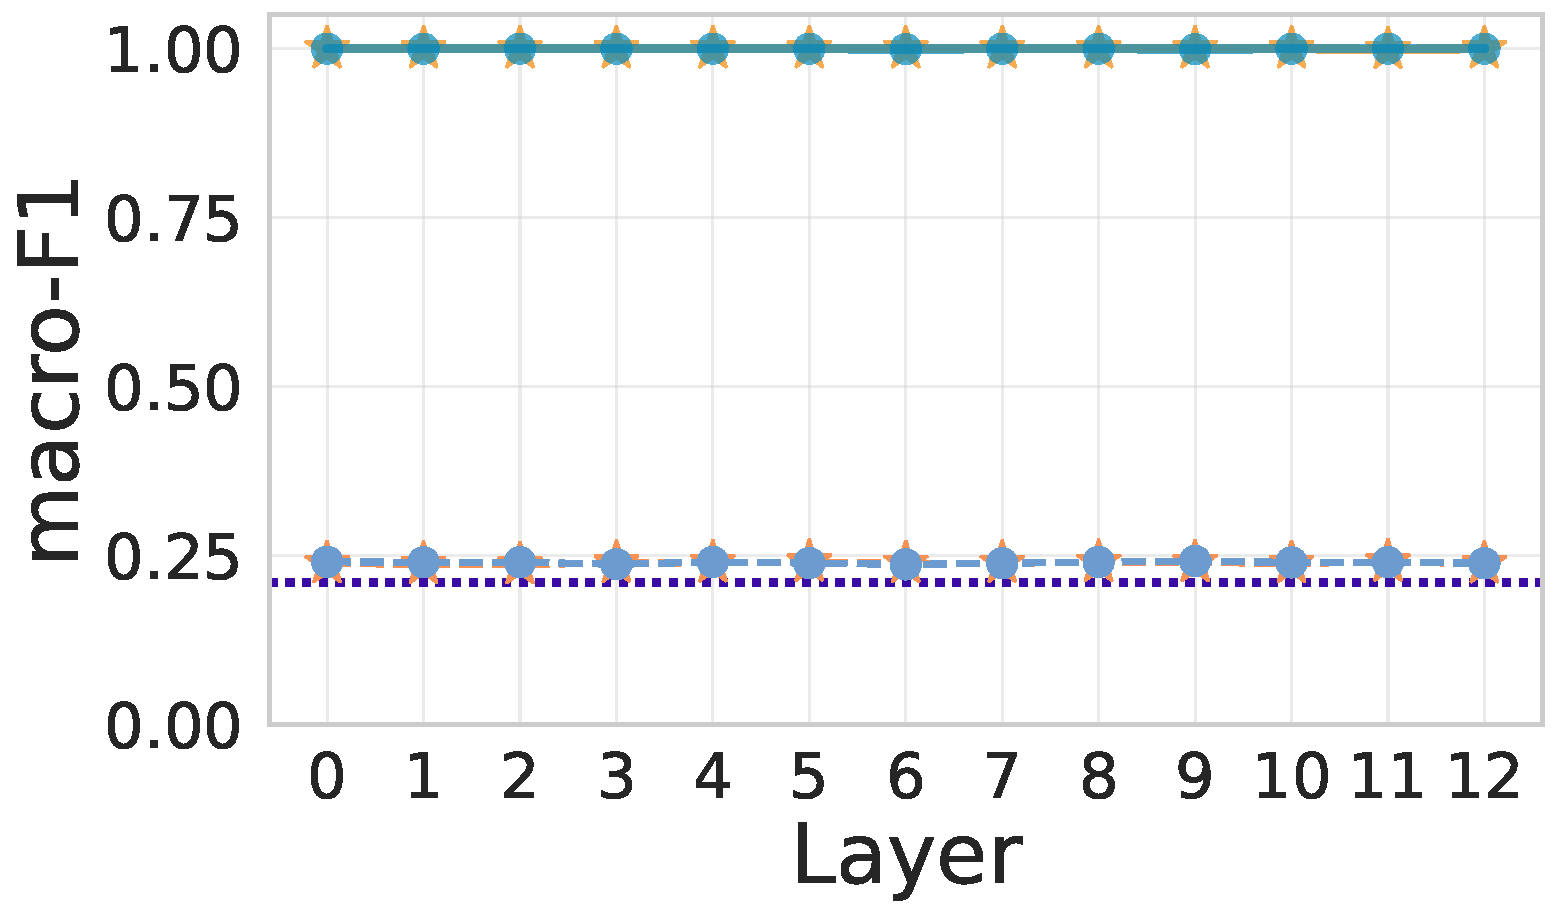
\includegraphics[width=\linewidth]{results_combined_f1/atom_type.pdf}
    \caption{atom type}
\end{subfigure}\hfill
\begin{subfigure}[t]{0.24\textwidth}
    \centering
    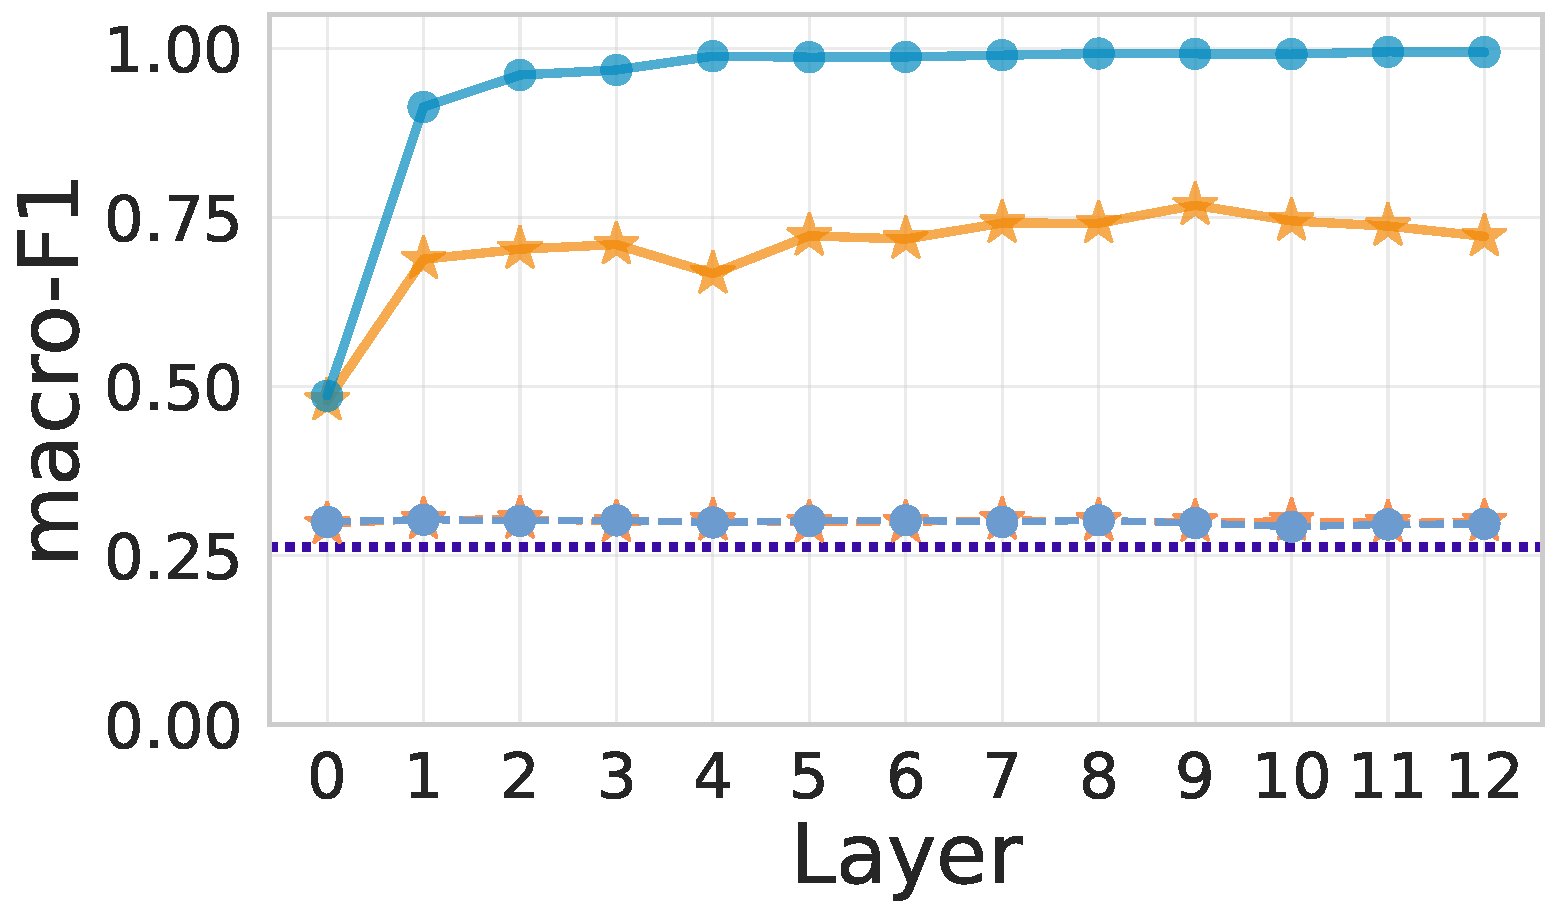
\includegraphics[width=\linewidth]{results_combined_f1/hybridization.pdf}
    \caption{hybridization}
\end{subfigure}\hfill
\begin{subfigure}[t]{0.24\textwidth}
    \centering
    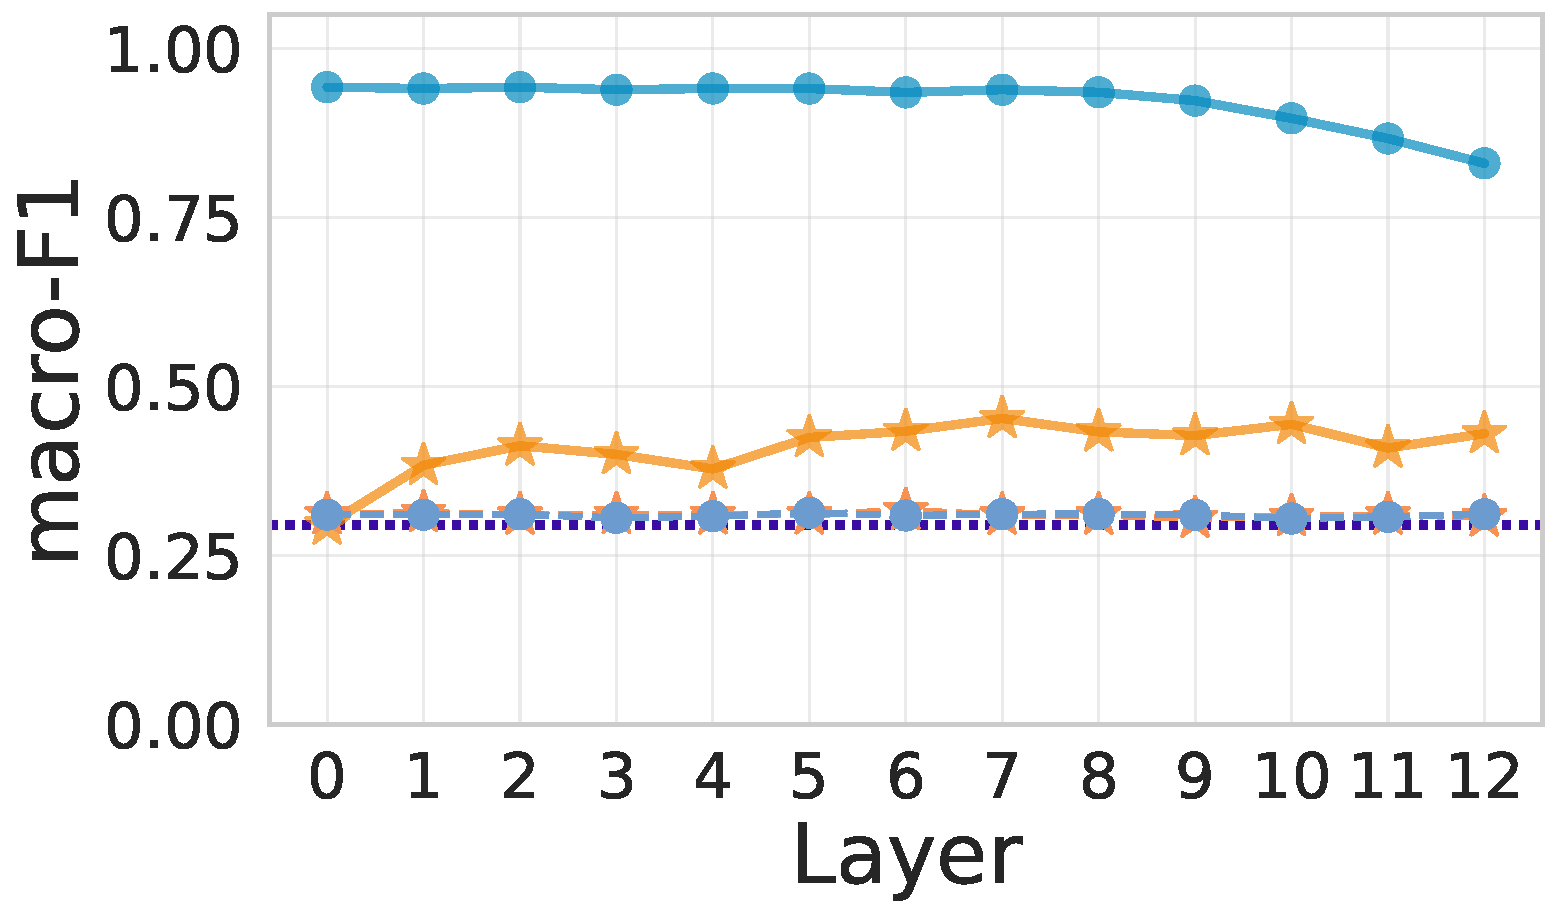
\includegraphics[width=\linewidth]{results_combined_f1/chiral_tag.pdf}
    \caption{chiral tag}
\end{subfigure}\hfill
\begin{subfigure}[t]{0.24\textwidth}
    \centering
    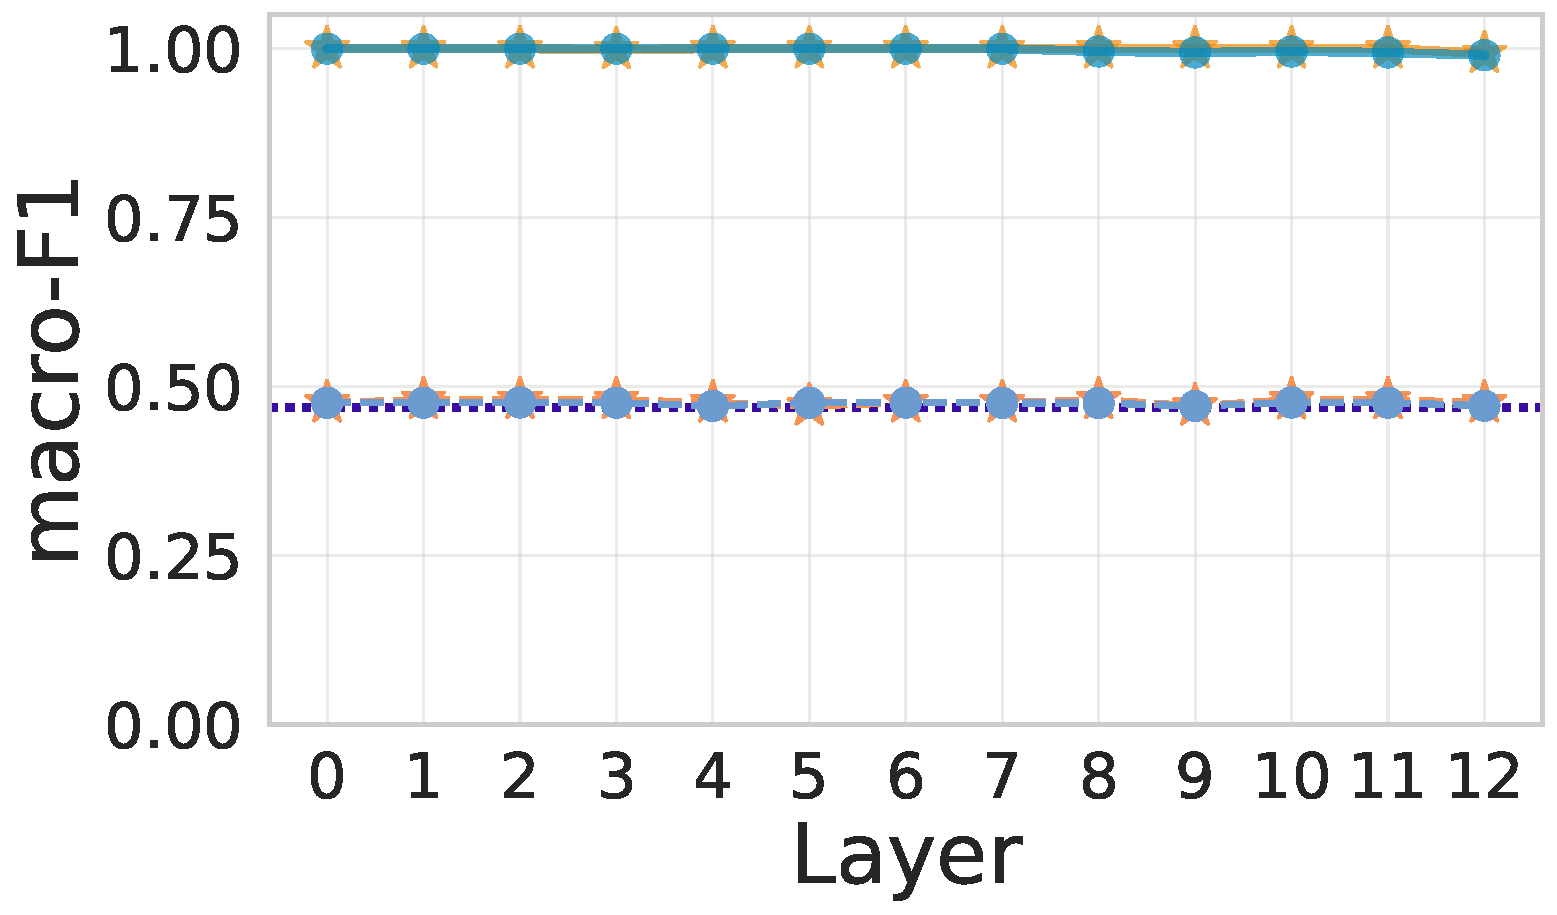
\includegraphics[width=\linewidth]{results_combined_f1/is_aromatic.pdf}
    \caption{is aromatic}
\end{subfigure}

\vspace{0.6em}

\begin{subfigure}[t]{0.24\textwidth}
    \centering
    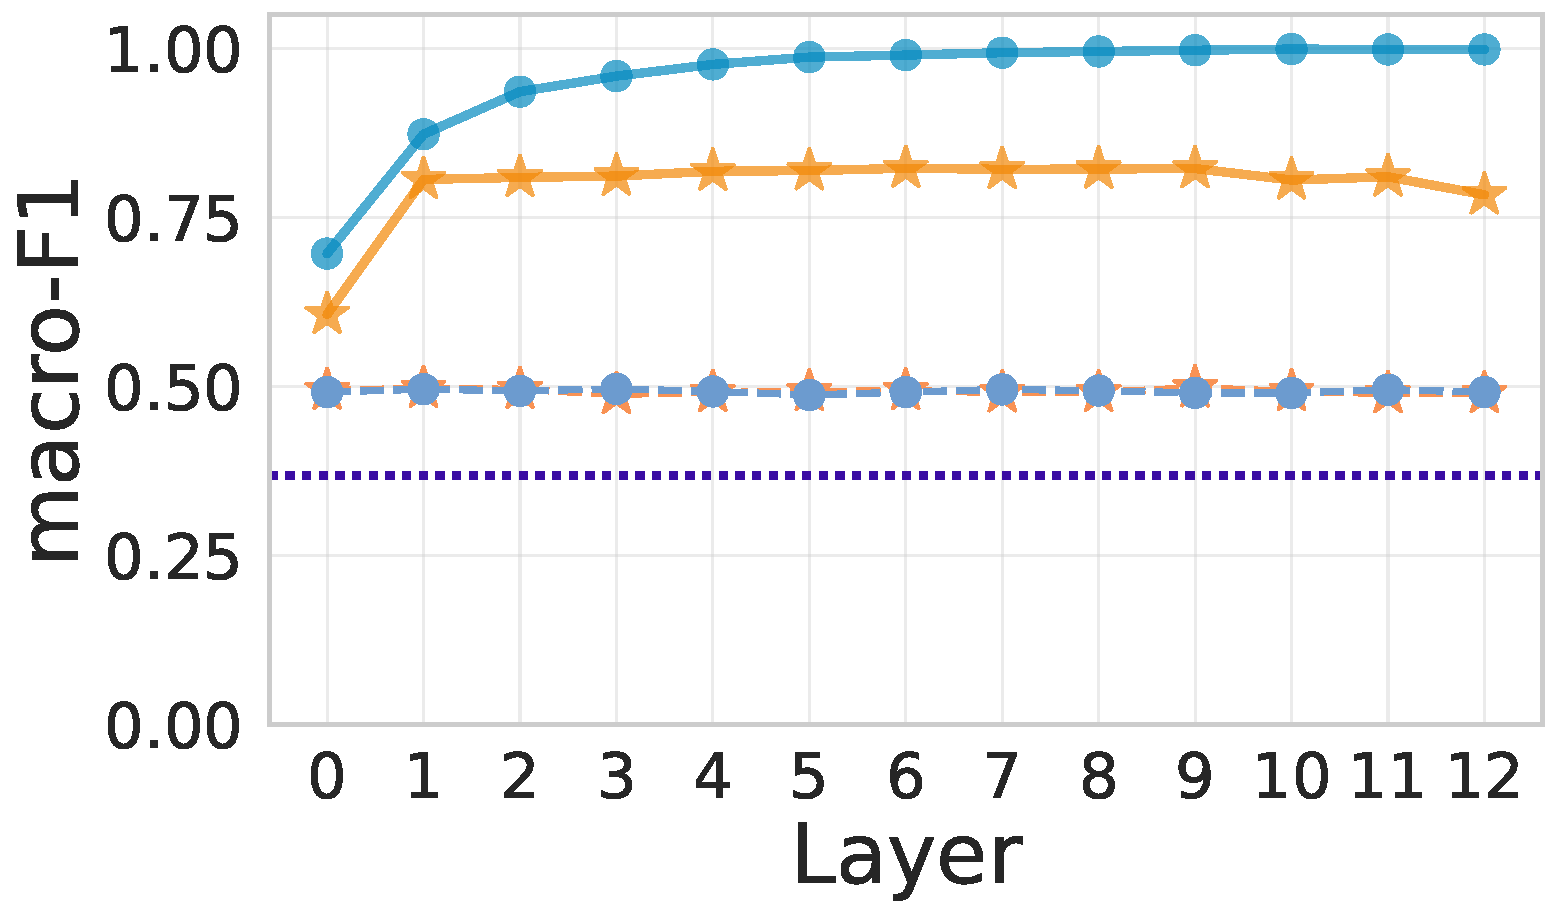
\includegraphics[width=\linewidth]{results_combined_f1/is_in_ring.pdf}
    \caption{is in ring}
\end{subfigure}\hfill
\begin{subfigure}[t]{0.24\textwidth}
    \centering
    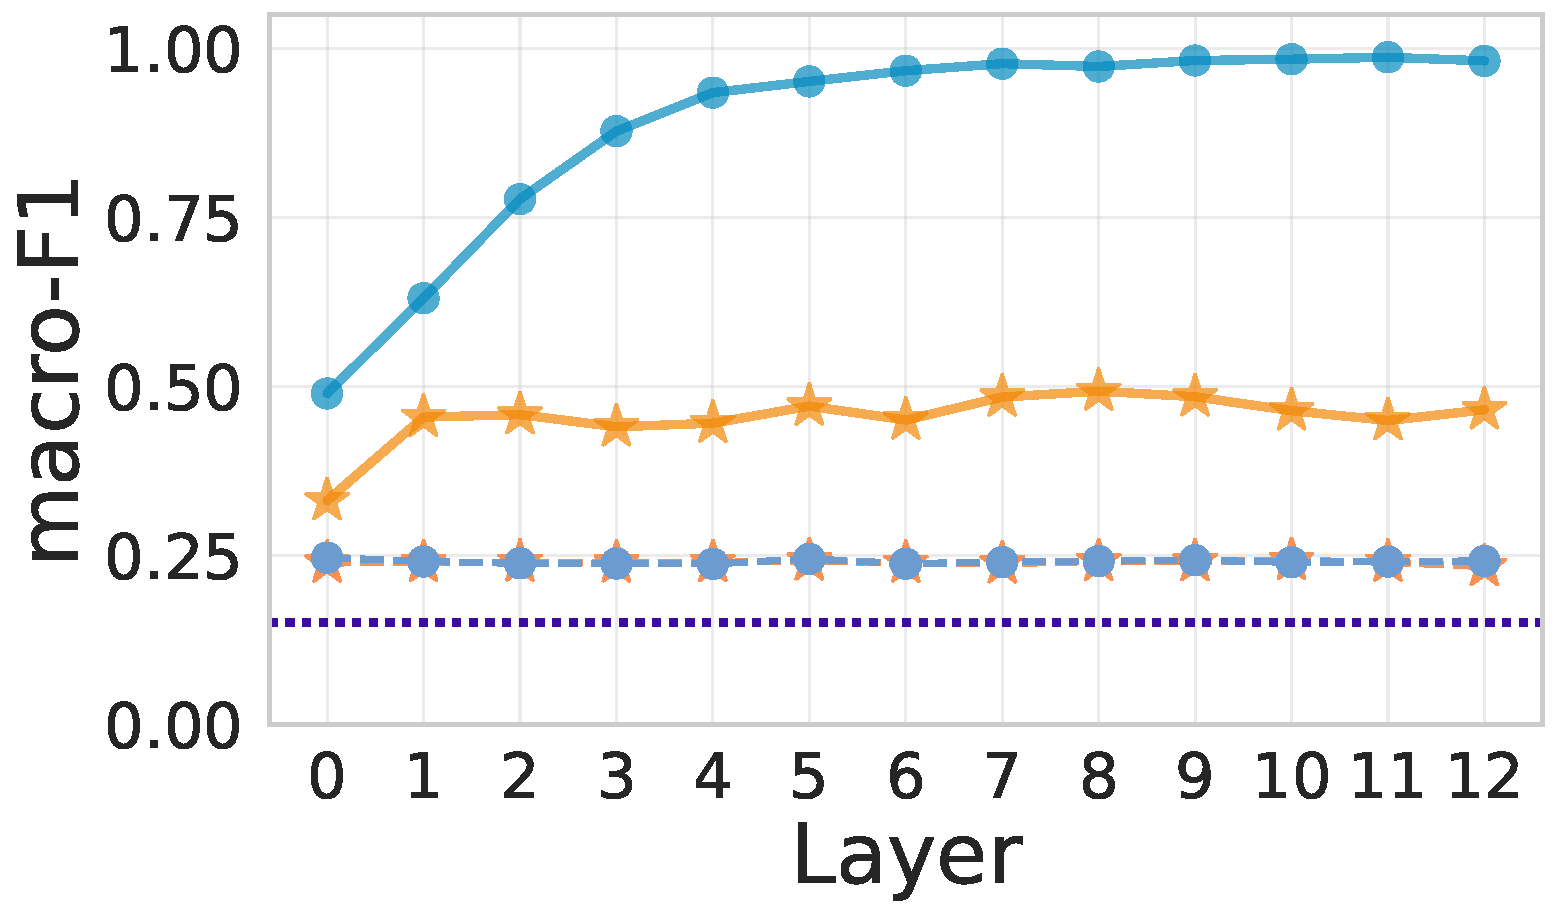
\includegraphics[width=\linewidth]{results_combined_f1/degree.pdf}
    \caption{degree}
\end{subfigure}\hfill
\begin{subfigure}[t]{0.24\textwidth}
    \centering
    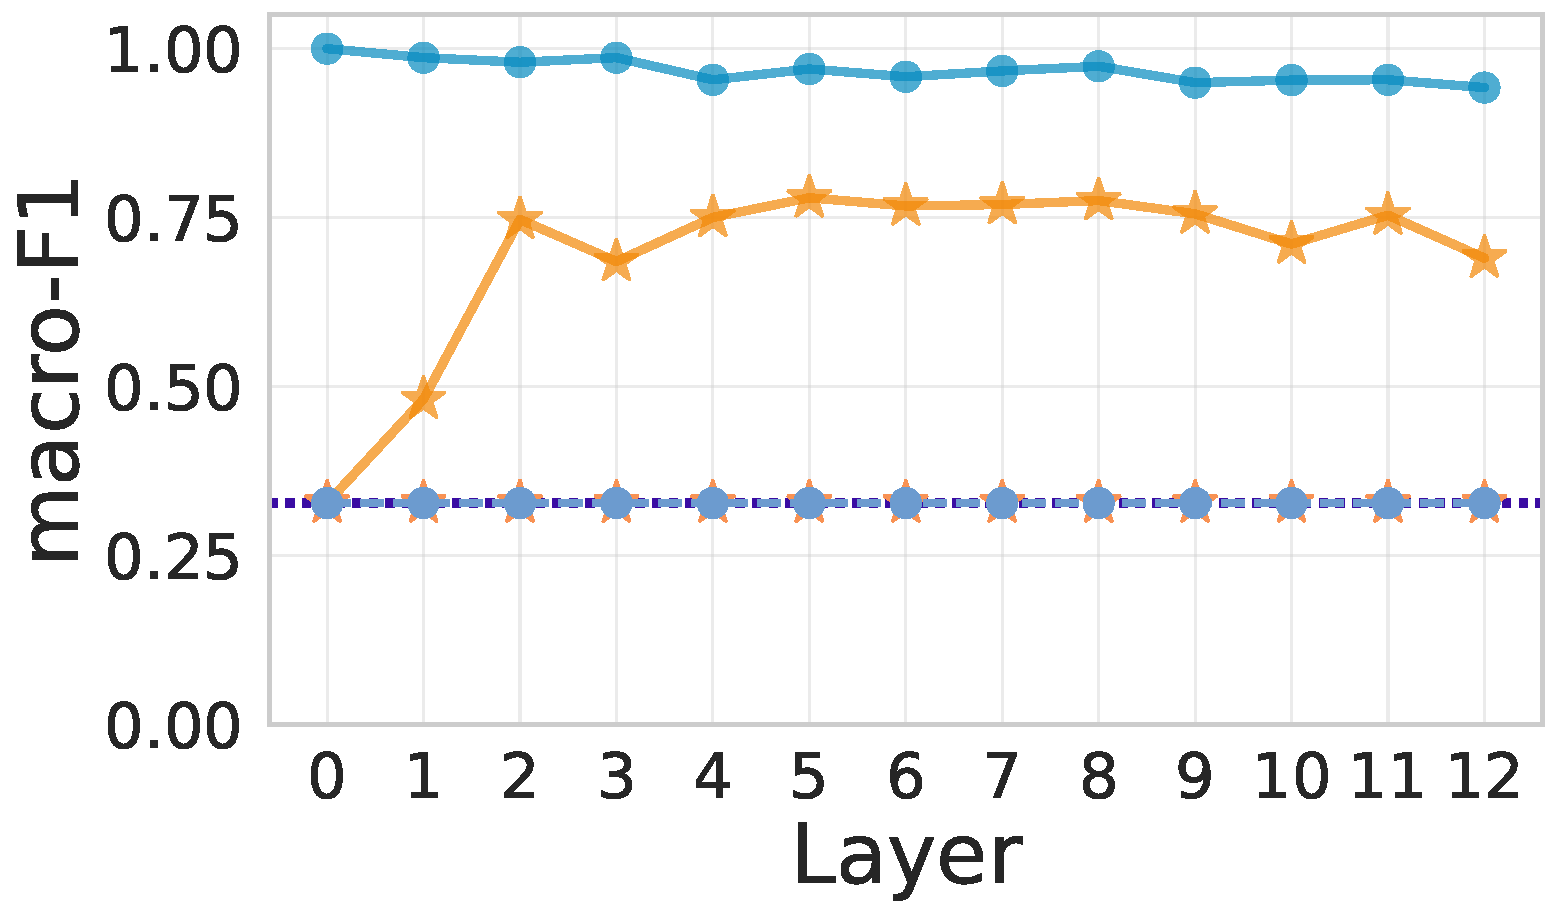
\includegraphics[width=\linewidth]{results_combined_f1/formal_charge.pdf}
    \caption{formal charge}
\end{subfigure}\hfill
\begin{subfigure}[t]{0.24\textwidth}
    \centering
    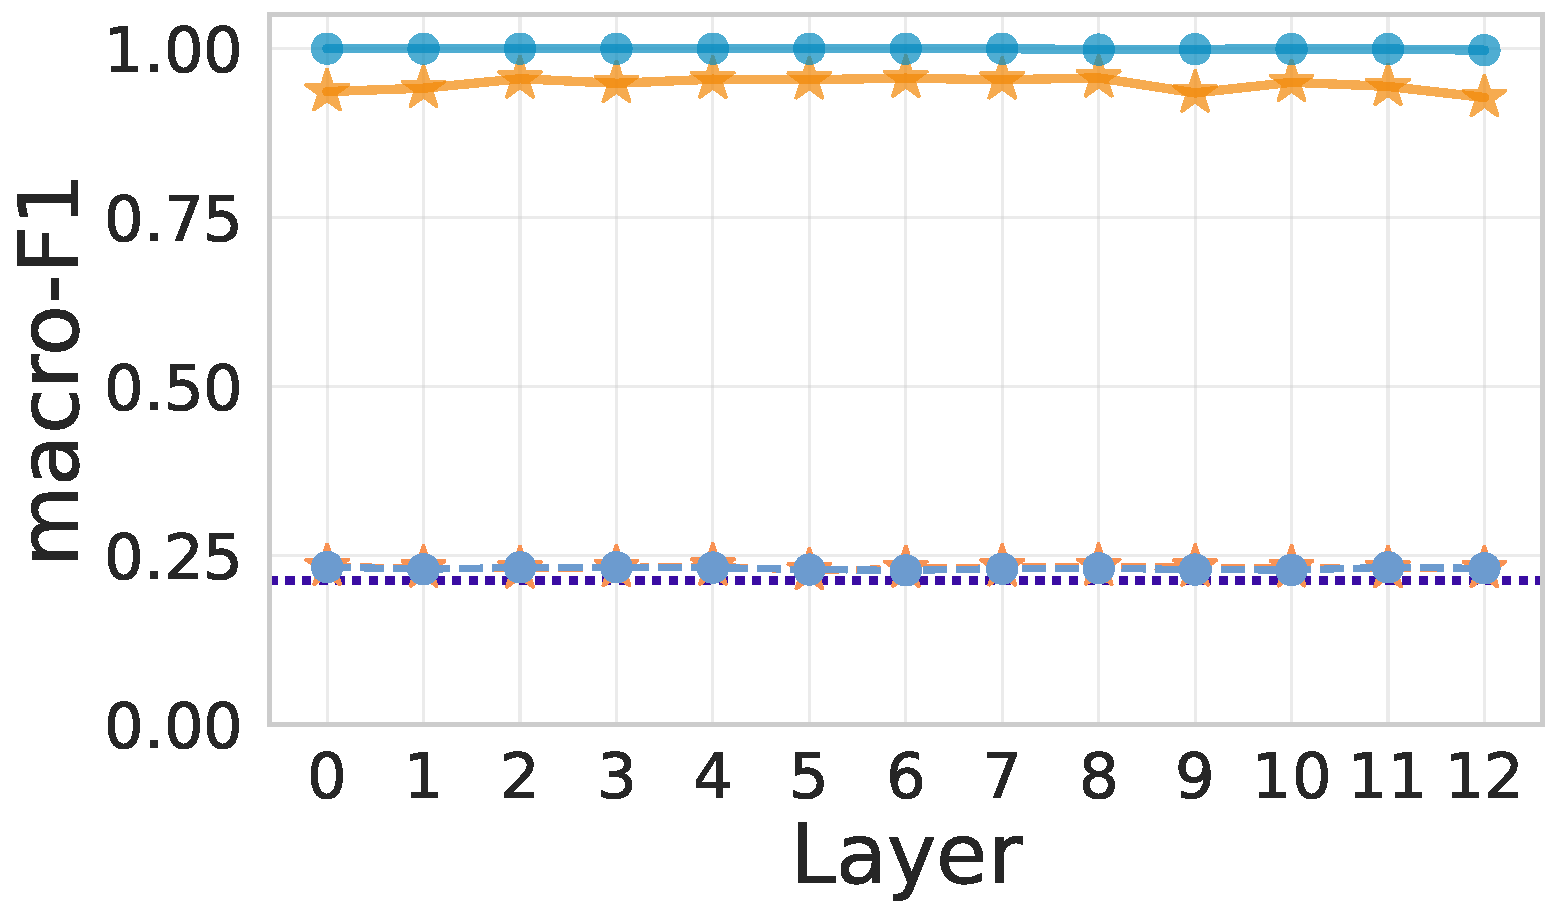
\includegraphics[width=\linewidth]{results_combined_f1/total_valence.pdf}
    \caption{total valence}
\end{subfigure}

\vspace{0.4em}

\centerline{\includegraphics[width=0.95\textwidth]{results_combined_f1/legend.pdf}}

\caption{Per-layer linear-probe macro-F1 on the same eight tasks. Under macro-F1 \smi vs.\ \molm gap on contextual tasks is more pronounced than under accuracy, because macro-F1 penalises probes that effectively predict the majority class.}
\label{fig:f1}
\end{figure*}

\para{MLP-probe control.} To test whether the linear probe is bottlenecked by lack of nonlinearity, we additionally train a 2-layer MLP $\mathrm{MLPProbe}(\mathbf{x}) = \mathbf{W}_2\,\mathrm{ReLU}(\mathbf{W}_1\,\mathbf{x} + \mathbf{b}_1) + \mathbf{b}_2$ with hidden size $128$ on the real hidden states. Across all eight tasks and both models, the MLP probe improves test accuracy over the linear probe by at most $0.03$ in absolute terms, with most improvements being $\leq 0.01$. The largest gain is on \molm{} hybridization ($+0.03$ accuracy / $+0.07$ macro-F1 at layer $5$); on surface-form tasks the gap is essentially zero. We conclude that the chemical properties under study are approximately linearly accessible from the residual stream, and the conclusions drawn from the linear probe are not artifacts of probe capacity.

\para{Random-features control.} For each (task, layer) pair we additionally train an identical linear probe on a Gaussian random-features matrix $\mathbf{X}_{\mathrm{rand}} \in \mathbb{R}^{N \times d}$ with i.i.d.\ entries $\mathcal{N}(0, 1)$, sampled once per script run and reused for every (task, layer). The same molecule-level split, class encoding, and standardization are applied; the probe sees the same atom labels but uninformative inputs. Test macro-F1 falls within $1$--$2$ percentage points of $1/C_\tau$ (the chance level under macro-F1 when always predicting the majority class) for every task on both models, confirming that the real-features probe accuracy reflects encoder structure rather than overfitting capacity in the linear head.

\para{Macro-F1.} Figure~\ref{fig:f1} reports per-layer macro-F1 for six tasks for which it is informative (we omit atom type and formal charge, where the majority baseline is at or near $1.0$ and macro-F1 saturates). Under macro-F1 the \smi{} vs.\ \molm{} gap on contextual tasks is more pronounced than under accuracy, because macro-F1 penalizes probes that effectively reproduce the majority-vote baseline on imbalanced classes.

\subsection{Probe accuracy and steering for the remaining four properties}

The main text shows aromaticity, ring membership, degree, and chiral tag. Figure~\ref{fig:acc-all} and Figure~\ref{fig:steer-layer-all} report linear-probe accuracy and intervention success rate for the four remaining properties: atom type, hybridization, formal charge, and total valence. Atom type and formal charge are surface-form (or near-surface-form, since the majority baseline of formal charge is already $0.97$): both models reach the same near-saturation accuracy at the embedding and layer-sweep success curves are dominated by probe-prototype geometry on the multi-class cycle target. Hybridization and total valence are contextual; \smi{} reaches near-perfect probe accuracy and intervention success by mid-layers, while \molm{} plateaus several points below on probing and lifts only at the deepest layers under intervention---the same shape we see for the contextual tasks in the main text.

\begin{figure}[t]
\centering
\begin{subfigure}[t]{0.24\linewidth}
    \centering
    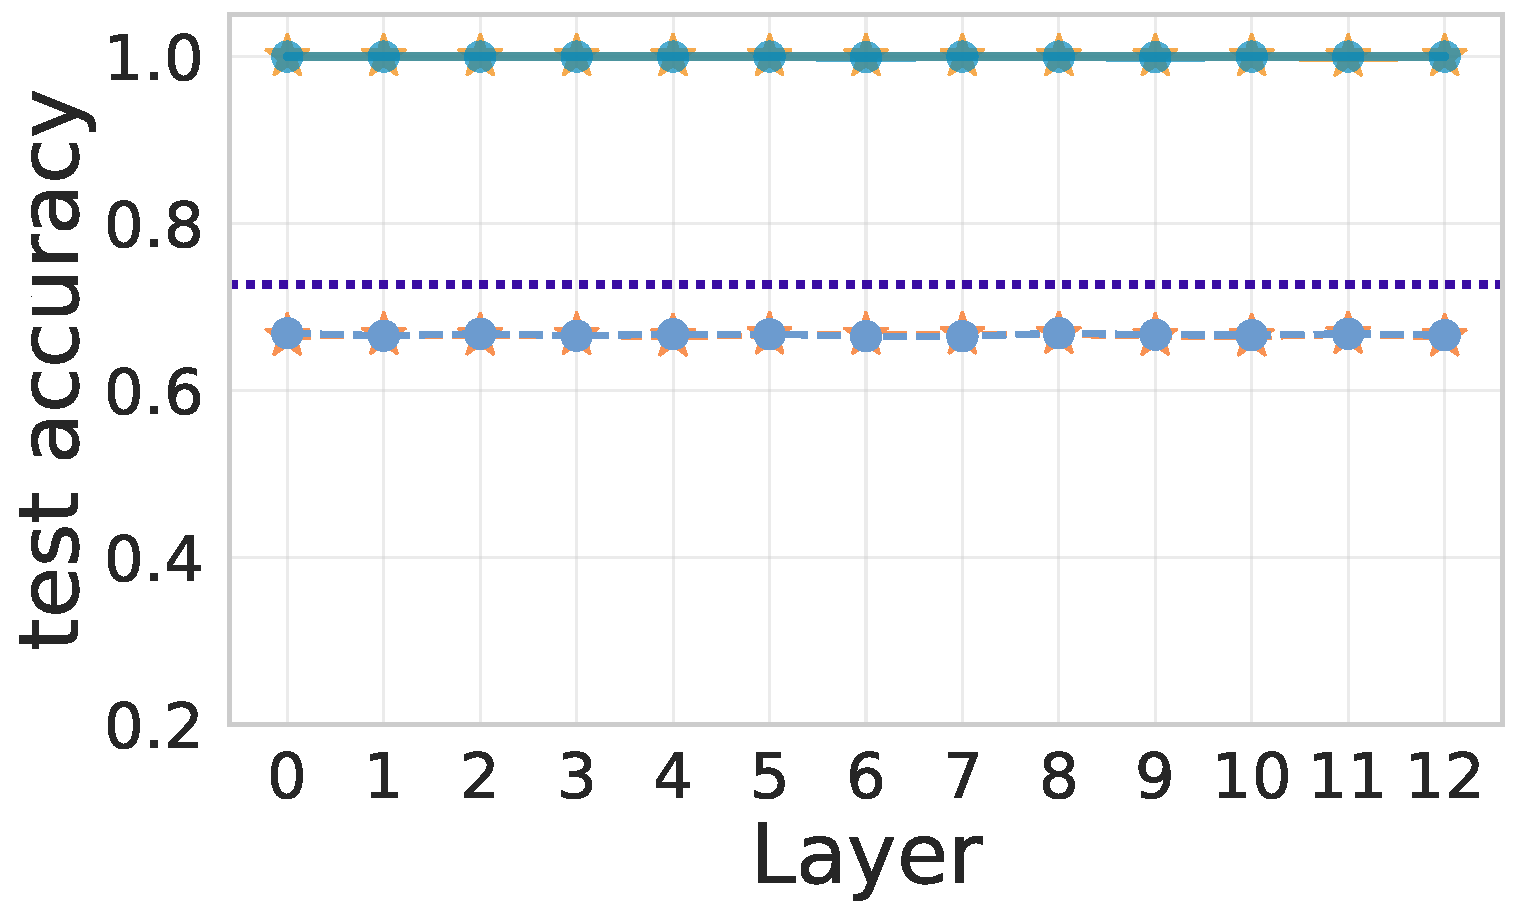
\includegraphics[width=\linewidth]{results_combined/atom_type.pdf}
    \subcaption{atom type}
    \label{fig:acc-all-atom-type}
\end{subfigure}\hfill
\begin{subfigure}[t]{0.24\linewidth}
    \centering
    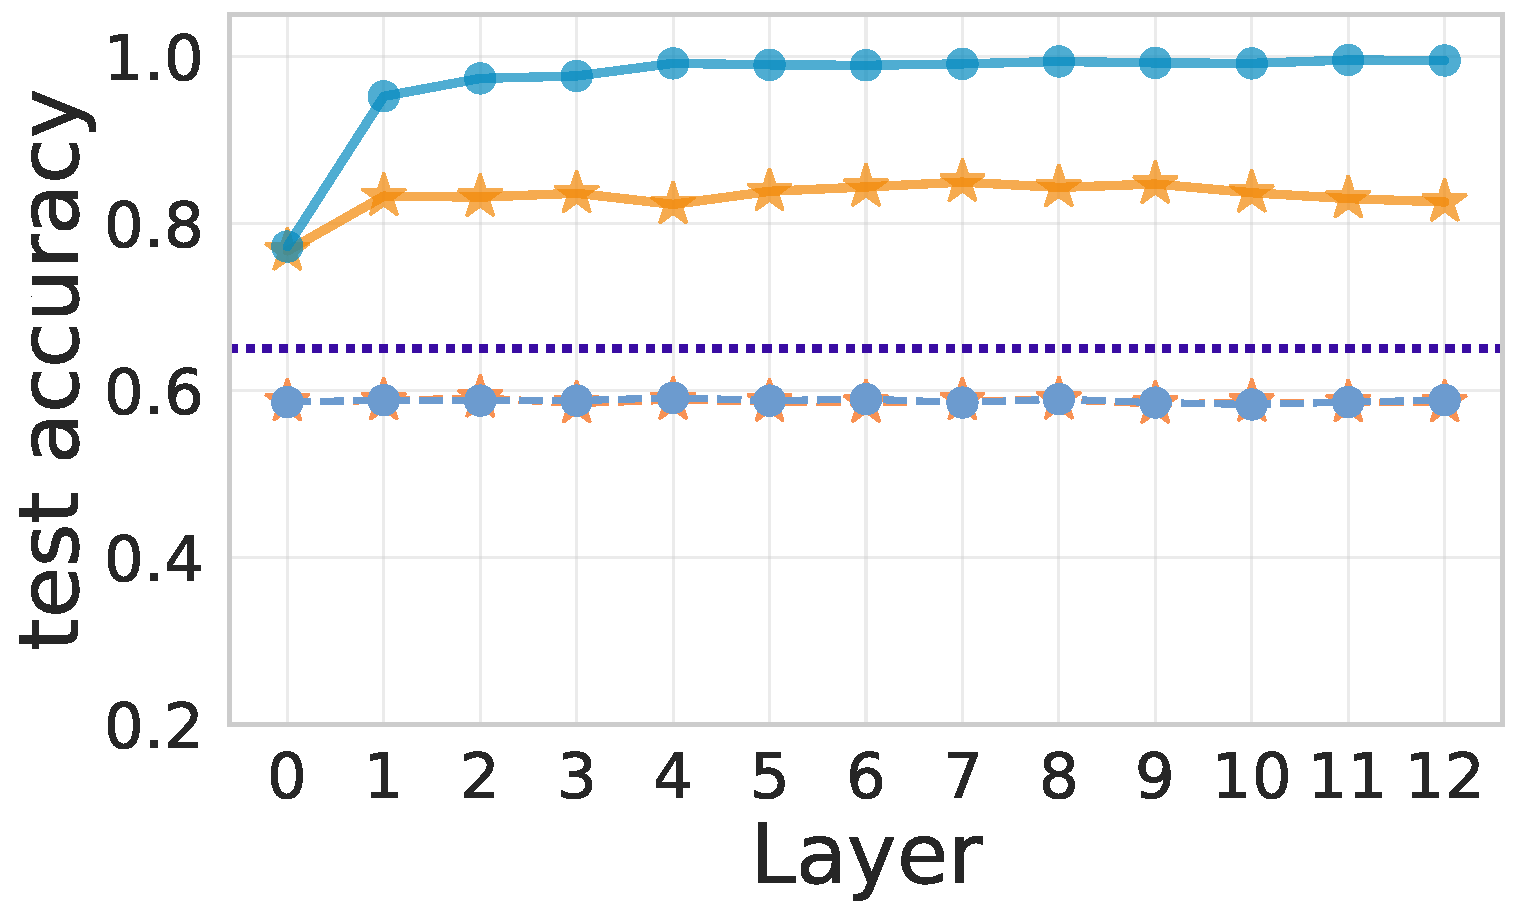
\includegraphics[width=\linewidth]{results_combined/hybridization.pdf}
    \subcaption{hybridization}
    \label{fig:acc-all-hybridization}
\end{subfigure}\hfill
\begin{subfigure}[t]{0.24\linewidth}
    \centering
    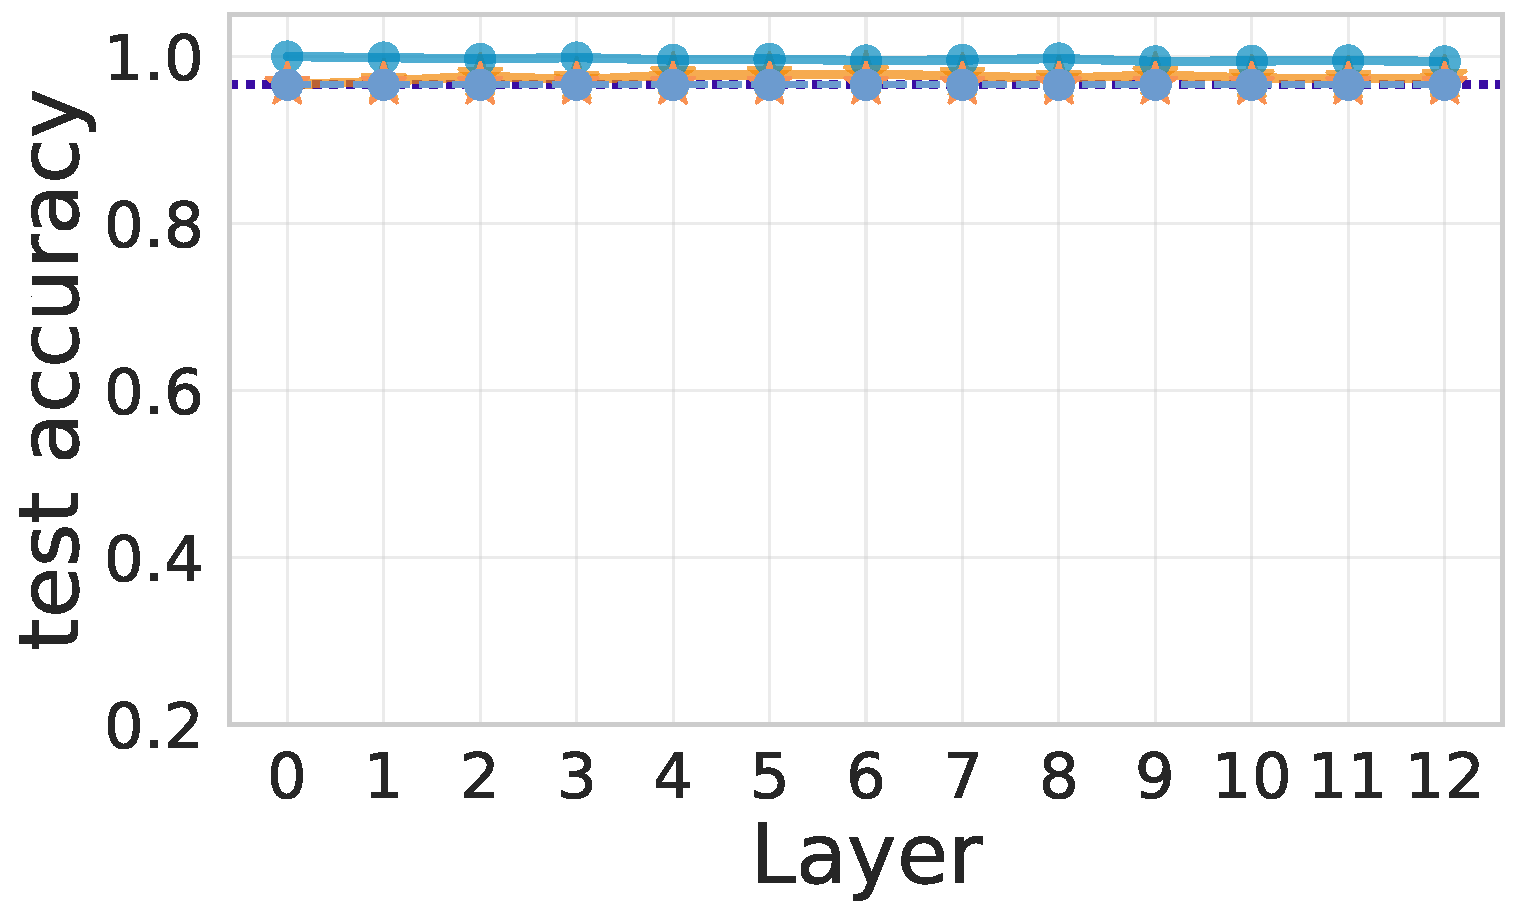
\includegraphics[width=\linewidth]{results_combined/formal_charge.pdf}
    \subcaption{formal charge}
    \label{fig:acc-all-formal-charge}
\end{subfigure}\hfill
\begin{subfigure}[t]{0.24\linewidth}
    \centering
    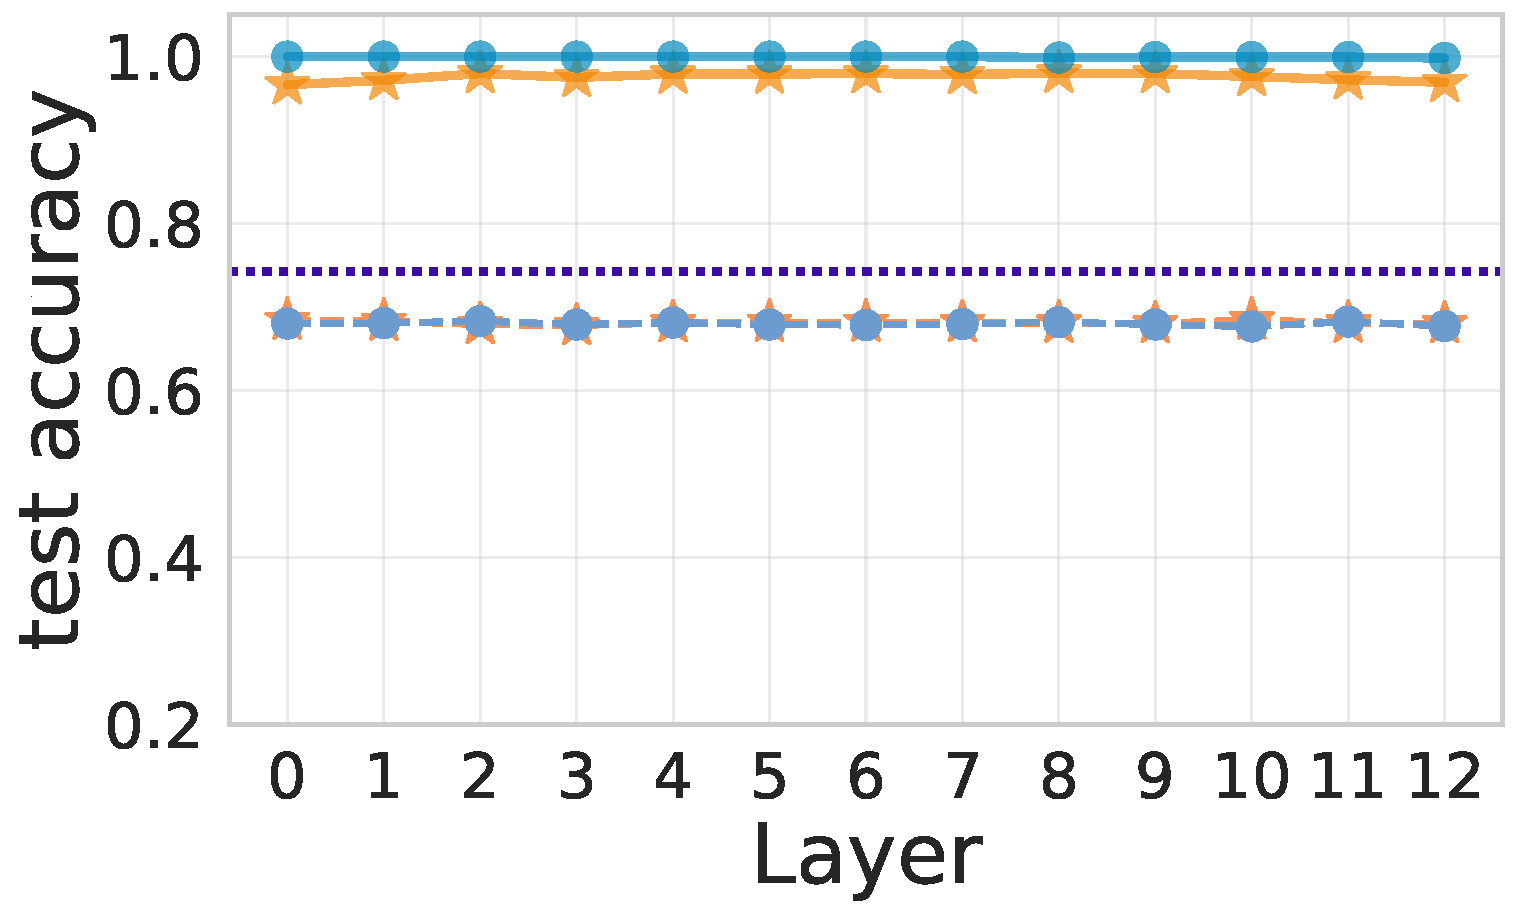
\includegraphics[width=\linewidth]{results_combined/total_valence.pdf}
    \subcaption{total valence}
    \label{fig:acc-all-total-valence}
\end{subfigure}

\vspace{0.4em}

\centerline{\includegraphics[width=0.85\linewidth]{results_combined/legend.pdf}}

\caption{Linear-probe test accuracy per layer for the four properties not shown in the main text. Atom type (\ref{fig:acc-all-atom-type}) is surface-form and saturates at $1.0$ from layer~$0$ in both models. Formal charge (\ref{fig:acc-all-formal-charge}) is similarly close to its $0.97$ majority baseline in both models from the embedding onward. Hybridization (\ref{fig:acc-all-hybridization}) and total valence (\ref{fig:acc-all-total-valence}) are contextual and follow the same pretraining-difference shape as ring membership, degree, and chiral tag in the main text: \smi reaches near-perfect accuracy by mid-layers while \molm plateaus several points below.}
\label{fig:acc-all}
\end{figure}
\begin{figure}[t]
\centering
\begin{subfigure}[t]{0.48\linewidth}
    \centering
    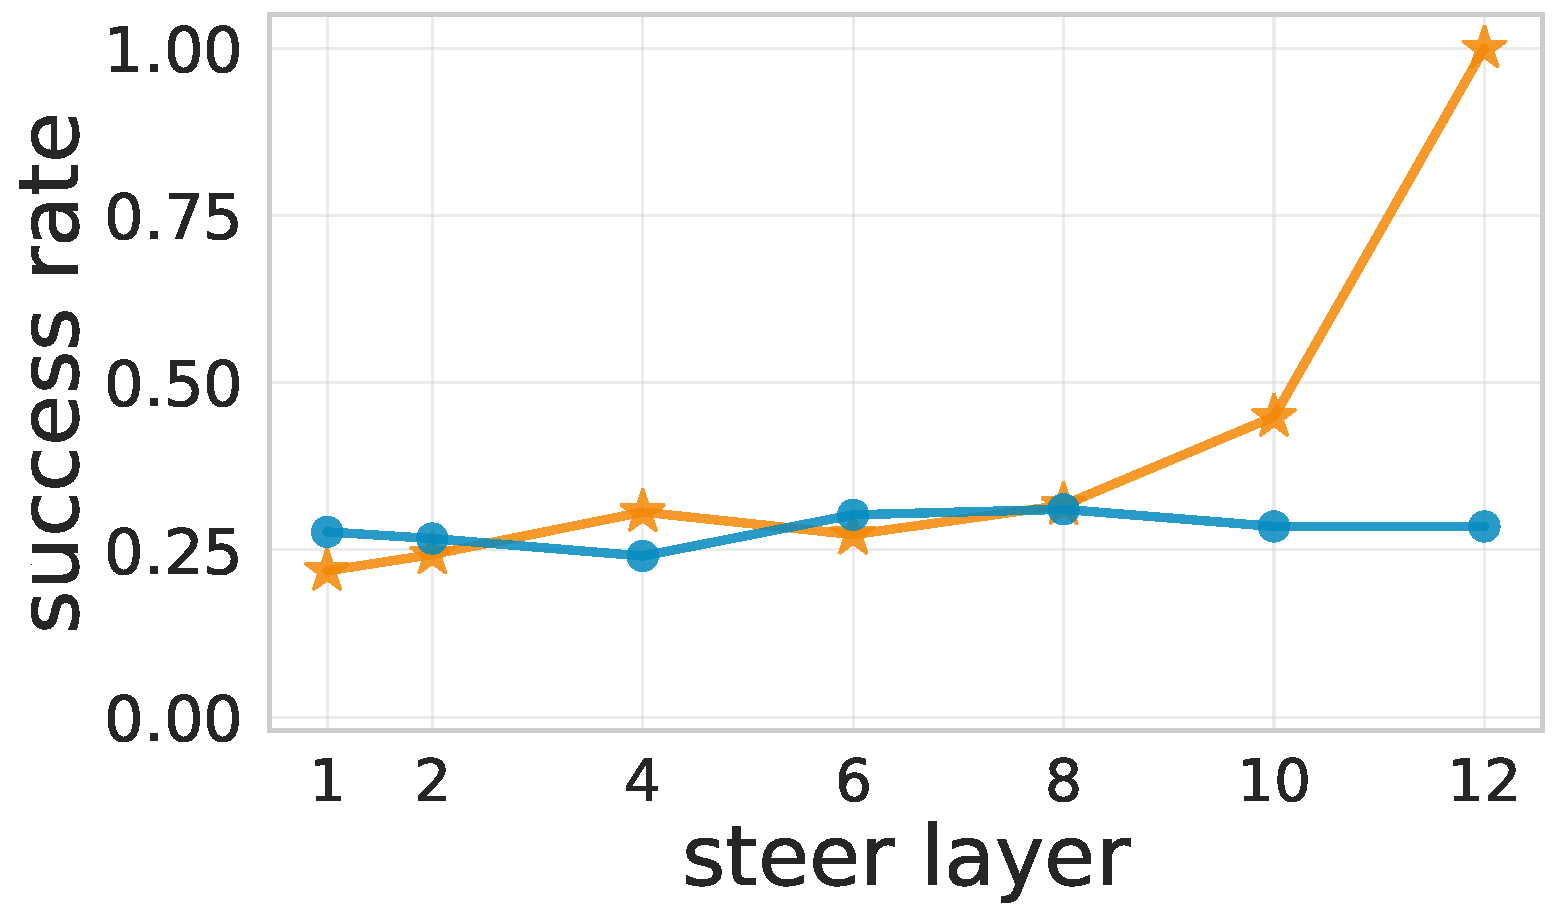
\includegraphics[width=\linewidth]{results_steer_layers/by_layer_atom_type.pdf}
    \subcaption{atom type}
    \label{fig:steer-all-atom-type}
\end{subfigure}\hfill
\begin{subfigure}[t]{0.48\linewidth}
    \centering
    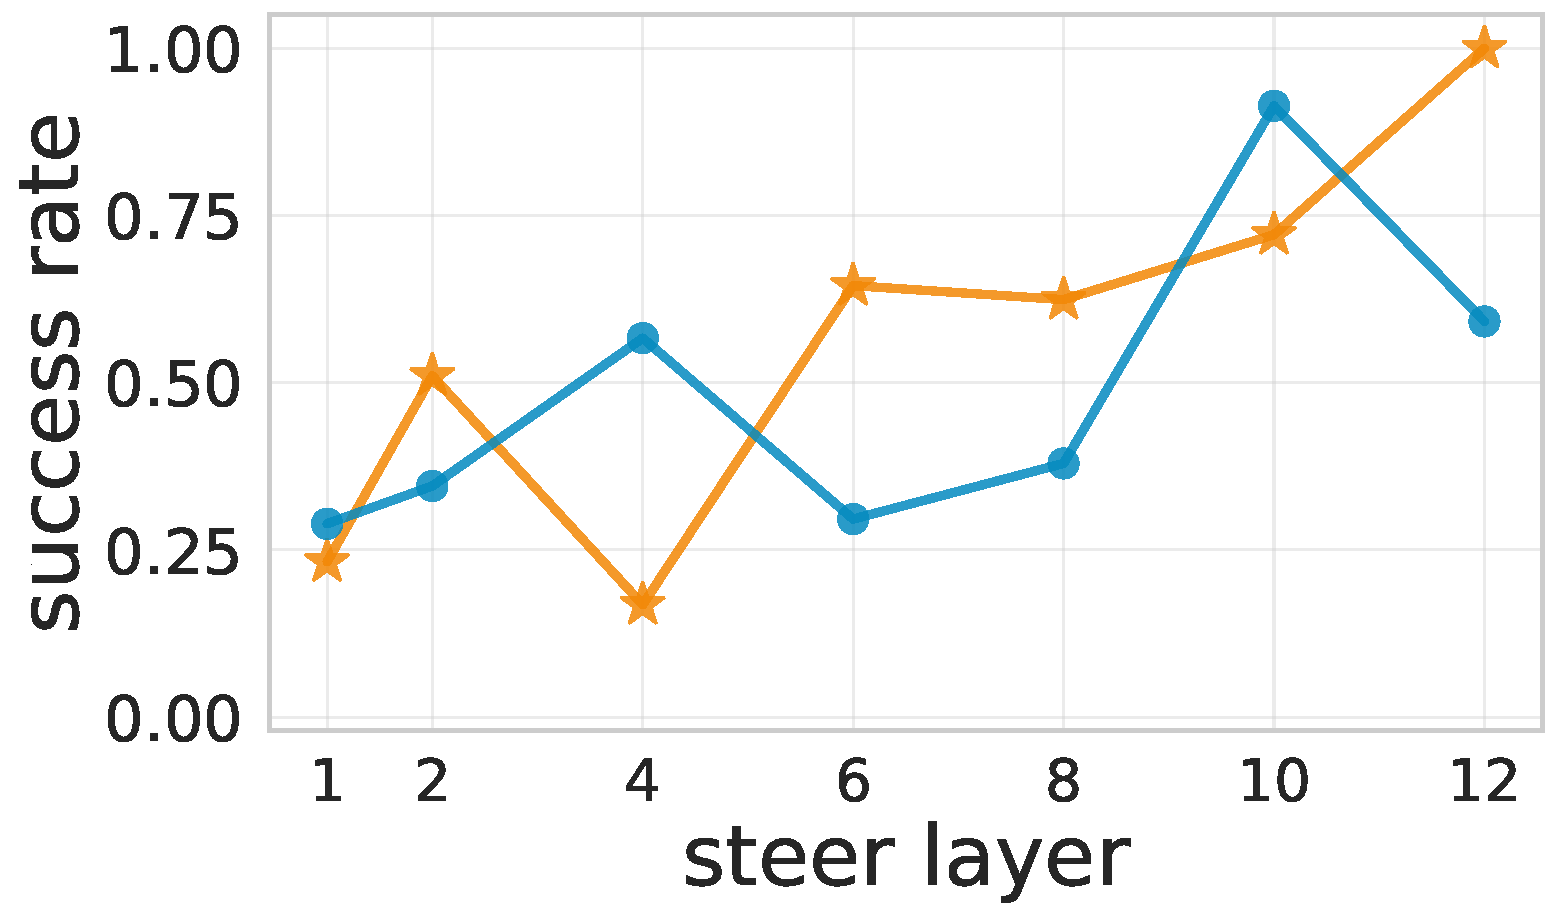
\includegraphics[width=\linewidth]{results_steer_layers/by_layer_hybridization.pdf}
    \subcaption{hybridization}
    \label{fig:steer-all-hybridization}
\end{subfigure}

\vspace{0.6em}

\begin{subfigure}[t]{0.48\linewidth}
    \centering
    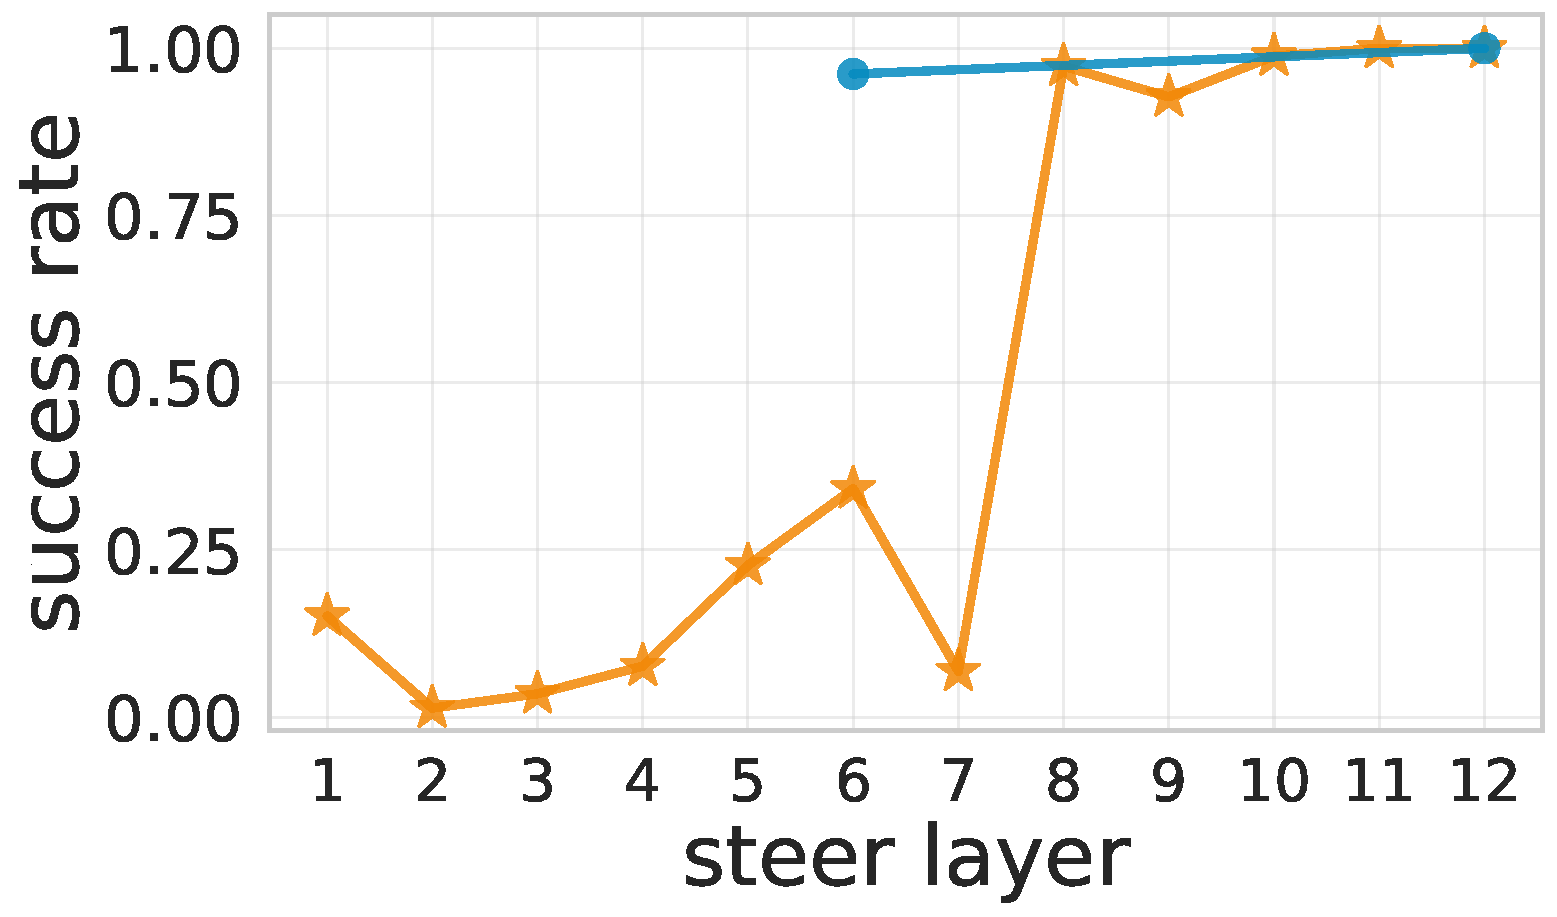
\includegraphics[width=\linewidth]{results_steer_layers/by_layer_formal_charge.pdf}
    \subcaption{formal charge}
    \label{fig:steer-all-formal-charge}
\end{subfigure}\hfill
\begin{subfigure}[t]{0.48\linewidth}
    \centering
    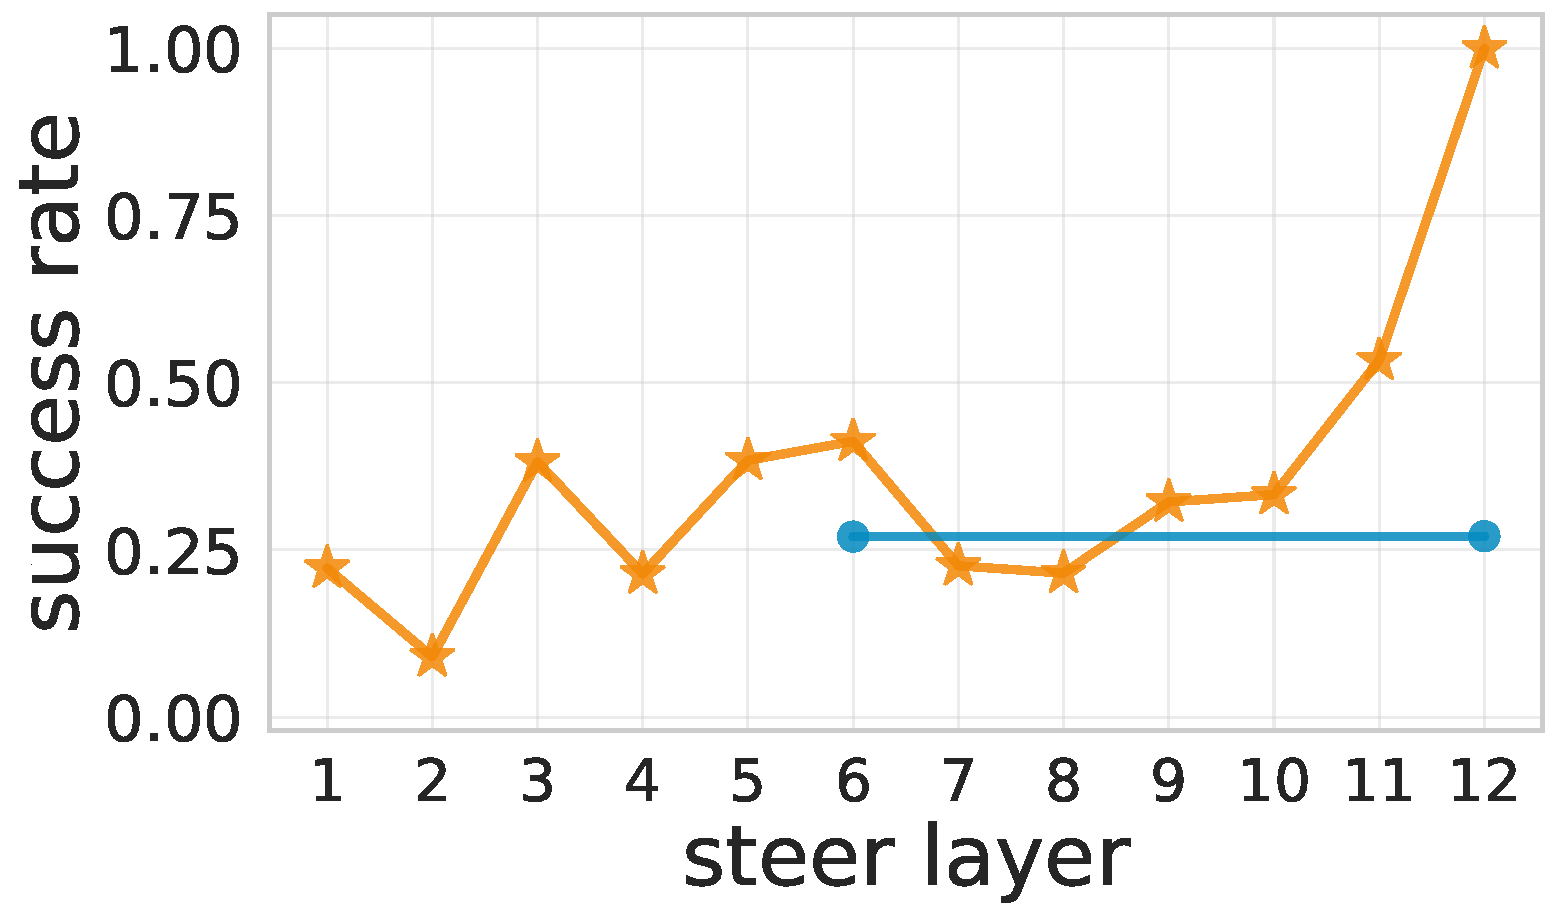
\includegraphics[width=\linewidth]{results_steer_layers/by_layer_total_valence.pdf}
    \subcaption{total valence}
    \label{fig:steer-all-total-valence}
\end{subfigure}

\vspace{0.4em}

\centerline{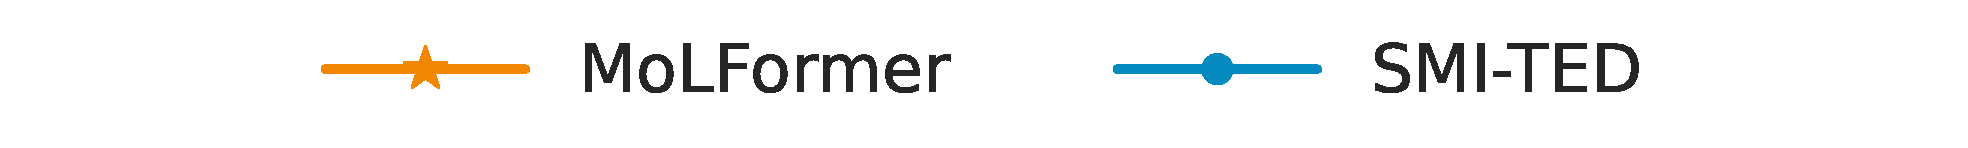
\includegraphics[width=0.5\linewidth]{results_steer_layers/by_layer_legend.pdf}}

\caption{Intervention success rate as a function of the steer layer for the four properties not shown in the main text. Formal charge (\ref{fig:steer-all-formal-charge}) follows the same pretraining-difference shape seen in the main text: \smi saturates at high success by mid-layers, \molm climbs gradually until the top of the encoder. Atom type (\ref{fig:steer-all-atom-type}), hybridization (\ref{fig:steer-all-hybridization}), and total valence (\ref{fig:steer-all-total-valence}) are multi-class targets and the cycle-target success rate is partly governed by the probe-prototype layout; we therefore additionally inspect the moved-off-source rate (Appendix~\ref{app:steering}) to disentangle ``the intervention had effect'' from ``the intervention hit the cycle target''.}
\label{fig:steer-layer-all}
\end{figure}


\subsection{Causal-steering setup}

\para{Steering vector.} For each (task, steer layer $\ell$) we form, in the original (unstandardized) hidden-state space,
\[
\mathbf{v}^{c \to c'} = (\mathbf{W}_{c'} - \mathbf{W}_{c}) / \boldsymbol{\sigma},
\]
where $\mathbf{W}_{c}$ is the layer-$\ell$ probe's row for class $c$ and $\boldsymbol{\sigma}$ is the per-feature training standard deviation. Adding $\alpha \cdot \mathbf{v}^{c \to c'}$ to a hidden state increases the standardized logit difference $\mathrm{logit}_{c'} - \mathrm{logit}_{c}$ by $\alpha \cdot \|\mathbf{W}_{c'} - \mathbf{W}_c\|_{\boldsymbol{\sigma}^{-2}}^2$. For binary tasks, $\mathrm{tgt} = 1 - \mathrm{src}$. For multi-class tasks, we use a cycle target $\mathrm{tgt} = (\mathrm{src} + 1) \bmod C_\tau$.

\para{Forward hook and intervention.} The hook is registered on the module that produces $\mathbf{h}^{(\ell)}$ (\texttt{model.encoder.layer[$\ell$-1]} for \molm{}, \texttt{encoder.blocks.layers[$\ell$-1]} for \smi{}), modifies that layer's output by adding the per-position steering tensor at atom-token positions only, and is removed in a \texttt{try/finally} block immediately after the post-intervention forward pass. The pre- and post-intervention forward passes are run with \texttt{output\_hidden\_states=True} to capture the residual stream at every depth.

\para{Layer sweep.} The main-text Figure~\ref{fig:steer-layer} and the appendix Figure~\ref{fig:steer-layer-all} sweep $\ell \in \{1, \ldots, 12\}$ and report, per (task, model, $\ell$), the intervention success rate at the best-performing $\alpha$ on held-out molecules. This best-$\alpha$-per-layer summary serves as a single scalar diagnostic of whether the encoder routes through the layer-$\ell$ probe direction.

\para{Metrics.} \emph{Intervention success rate} (or \emph{flip-to-target rate}) is the fraction of atom-token positions whose layer-$12$ probe prediction equals the intended target $c'$ after the intervention. We additionally track \emph{moved-off-source rate} (the fraction whose post-intervention layer-$12$ prediction differs from the source class $c$) so that, for multi-class tasks, ``the steering had effect'' can be disentangled from ``the steering hit the cycle target''---a distinction that matters when the cycle direction $\mathbf{W}_{c'} - \mathbf{W}_{c}$ does not point at the cycle-target centroid in the probe's prototype layout.

\para{Sample size and hyperparameters.} Each task is evaluated on $200$ molecules ($\sim 1.7$k atom-token positions; $197$ molecules and $1{,}719$ atom-token positions survive token-atom alignment) drawn from the QM9 partition not used for probe training. The $\alpha$ grid is $\{0, 1, 3, 10, 30, 100, 300\}$; the smallest non-zero $\alpha$ that maximizes success rate is reported per layer.
